\chapter{Simulation Results}

Both methods were tested in Octave at -3dB, 0dB, 3dB, 5dB, 10dB, and 15dB SNR. 
As test data, AM, Single Side Band AM, FM, BPSK, QAM, 16QAM, and 64QAM data was
used.  Each signal was modulated at 2048Hz and sampled at 8192Hz with complex
sampling being used.  This resulted in an over sampling rate of four.  For each
of the digital modulation schemes, a symbol rate equal to the center frequency
of 2048Hz was used.  For the analog modulated signals, white noise was filtered
to a bandwidth of 2048Hz as the input signal.  The FM frequency deviation was
set to 50Hz.

\section{Cumulant Method}

While \cite{swami2000} does not cover FM Modulation, an FM signal in the IQ
domain can be seen has a rotating phasor which given that the Cumulant Method is
phase invariant should result in the classification of M-PSK signal with M
approaching infinity.  
For the AM and SSB AM, data with an SNR of 1000dB was sent through the
classifier to determine the theoretical values of $|C40|$ and $C42$.  For AM,
$|C40|$ and $C42$ were $0.040723$ while SSB data had $|C40| = 0.079237$ and
$C42 = 0$.
The cumulant algorithm works in the time domain and assumes that the signal of
interest has been shifted to baseband.  Prior to running each of the data sets
through the cumulant algorithm, the signal was first frequency shifted to
baseband and then down sampled by a factor of four.  The signal was then sent
into the Cumulant algorithm for classification.  For each of the modulation
types, each correct hit as well as each false positive was noted.  For each
SNR level, one hundred tests were run for each of the modulation types.  
The number of data points used was varied and the outcome of each test case is
shown in tables \ref{tab:cumHit100pt} - \ref{tab:cumFalsePositive10000pt}.  The
number of data points takes into account the down sampling, ie. if 1000 data
points were used for the Cumulant algorithm, 4000 data points had been down
sampled.
Based on the observed simulated results, the Cumulant method performs fairly
well with limited data points.  The algorithm tends to favor the higher modulation
scheme of QAM64 when given an amplitude modulated data set and a large number of
data points.  The Cumulant method has the most difficulty with the QAM16 dataset
and would regularly classify it as QAM64.

\begin{table}
\caption{Cumulant Results, Hits: 100 data Points}
\centering
\begin{tabular}{ l | c | c | c | c | c | c } \hline
SNR   &	 -3 &	 0 &	 3 &	 5 &	 10 &	 15\\ \hline \hline 
AM    &	 3 &	 19 &	 29 &	 31 &	 60 &	 99 \\ \hline 
SSB   &	 86 &	 78 &	 79 &	 79 &	 86 &	 91 \\ \hline 
FM    &	 0 &	 0 &	 0 &	 0 &	 0 &	 0 \\ \hline 
BPSK  &	 0 &	 0 &	 0 &	 0 &	 100 &	 100 \\ \hline 
QAM   &	 0 &	 0 &	 0 &	 0 &	 36 &	 100 \\ \hline 
QAM16 &	 0 &	 0 &	 0 &	 2 &	 35 &	 98 \\ \hline 
QAM64 &	 11 &	 26 &	 45 &	 81 &	 99 &	 100 \\ \hline 
\end{tabular}
\label{tab:cumHit100pt}
\end{table}

\begin{table}
\caption{Cumulant Results, False Positives: 100 data Points}
\centering
\begin{tabular}{ l | c | c | c | c | c | c } \hline
SNR   &	 -3 &	 0 &	 3 &	 5 &	 10 &	 15\\ \hline \hline 
AM &	 1.6 &	 1.4 &	 0.7 &	 0.4 &	 0.0 &	 0.0 \\ \hline 
SSB &	 62.6 &	 40.0 &	 21.9 &	 12.9 &	 5.7 &	 0.1 \\ \hline 
FM &	 0.1 &	 0.3 &	 0.4 &	 0.6 &	 0.1 &	 0.0  \\ \hline 
BPSK &	 0.0 &	 0.0 &	 0.0 &	 0.0 &	 0.1 &	 14.3 \\ \hline 
QAM &	 0.0 &	 0.0 &	 13.4 &	 28.1 &	 14.1 &	 0.0 \\ \hline 
QAM16 &	 0.1 &	 3.7 &	 12.6 &	 1.9 &	 9.1 &	 0.0 \\ \hline 
QAM64 &	 21.3 &	 37.0 &	 29.1 &	 28.6 &	 11.3 &	 1.6 \\ \hline
\end{tabular}
\label{tab:cumFalsePositive100pt}
\end{table}


\begin{table}
\caption{Cumulant Results, Hits: 1,000 data Points}
\centering
\begin{tabular}{ l | c | c | c | c | c | c } \hline
SNR   &	 -3 &	 0 &	 3 &	 5 &	 10 &	 15\\ \hline \hline 
AM    &	 9 &	 20 &	 20 &	 39 &	 75 &	 95 \\ \hline 
SSB   &	 81 &	 81 &	 81 &	 95 &	 99 &	 100 \\ \hline 
FM    &	 0 &	 0 &	 8 &	 96 &	 100 &	 100 \\ \hline 
BPSK  &	 0 &	 0 &	 0 &	 0 &	 100 &	 100 \\ \hline 
QAM   &	 0 &	 0 &	 0 &	 0 &	 4 &	 100 \\ \hline 
QAM16 &	 0 &	 0 &	 0 &	 0 &	 0 &	 33 \\ \hline 
QAM64 &	 0 &	 0 &	 5 &	 93 &	 100 &	 100 \\ \hline 
\end{tabular}
\label{tab:cumHit1000pt}
\end{table}

\begin{table}
\caption{Cumulant Results, False Positives: 1,000 data Points}
\centering
\begin{tabular}{ l | c | c | c | c | c | c } \hline
SNR   &	 -3 &	 0 &	 3 &	 5 &	 10 &	 15\\ \hline \hline 
AM &	 3.0 &	 2.7 &	 2.7 &	 0.7 &	 0.1 &	 0.0 \\ \hline 
SSB &	 83.9 &	 68.0 &	 45.6 &	 10.0 &	 3.6 &	 0.7 \\ \hline 
FM &	 0.0 &	 0.0 &	 0.0 &	 0.0 &	 0.0 &	 0.0  \\ \hline 
BPSK &	 0.0 &	 0.0 &	 0.0 &	 0.0 &	 0.0 &	 0.0 \\ \hline 
QAM &	 0.0 &	 0.0 &	 13.1 &	 14.3 &	 0.0 &	 0.0 \\ \hline 
QAM16 &	 0.0 &	 0.0 &	 1.1 &	 0.0 &	 13.7 &	 0.0 \\ \hline 
QAM64 &	 0.3 &	 14.9 &	 21.1 &	 28.9 &	 14.3 &	 9.6 \\ \hline
\end{tabular}
\label{tab:cumFalsePositive1000pt}
\end{table}

 
\begin{table}
\caption{Cumulant Results, Hits: 10,000 data Points}
\centering
\begin{tabular}{ l | c | c | c | c | c | c } \hline
SNR   &	 -3 &	 0 &	 3 &	 5 &	 10 &	 15\\ \hline \hline 
AM    &	 46 &	 61 &	 72 &	 83 &	 100 &	 100 \\ \hline 
SSB   &	 54 &	 59 &	 62 &	 70 &	 93 &	 100 \\ \hline 
FM    &	 0 &	 0 &	 0 &	 100 &	 100 &	 100 \\ \hline 
BPSK  &	 0 &	 0 &	 0 &	 0 &	 100 &	 100 \\ \hline 
QAM   &	 0 &	 0 &	 0 &	 0 &	 0 &	 100 \\ \hline 
QAM16 &	 0 &	 0 &	 0 &	 0 &	 0 &	 0 \\ \hline 
QAM64 &	 0 &	 0 &	 0 &	 100 &	 100 &	 100 \\ \hline 
\end{tabular}
\label{tab:cumHit10000pt}
\end{table}

\begin{table}
\caption{Cumulant Results, False Positives: 10,000 data Points}
\centering
\begin{tabular}{ l | c | c | c | c | c | c } \hline
SNR   &	 -3 &	 0 &	 3 &	 5 &	 10 &	 15\\ \hline \hline 
AM &	 6.6 &	 5.9 &	 5.4 &	 4.3 &	 1.0 &	 0.0 \\ \hline 
SSB &	 79.1 &	 62.7 &	 46.7 &	 2.4 &	 0.0 &	 0.0 \\ \hline 
FM &	 0.0 &	 0.0 &	 0.0 &	 0.0 &	 0.0 &	 0.0  \\ \hline 
BPSK &	 0.0 &	 0.0 &	 0.0 &	 0.0 &	 0.0 &	 0.0 \\ \hline 
QAM &	 0.0 &	 0.0 &	 14.3 &	 14.3 &	 0.0 &	 0.0 \\ \hline 
QAM16 &	 0.0 &	 0.0 &	 0.0 &	 0.0 &	 14.3 &	 0.0 \\ \hline 
QAM64 &	 0.0 &	 14.3 &	 14.4 &	 28.6 &	 14.3 &	 14.3 \\ \hline 
\end{tabular}
\label{tab:cumFalsePositive10000pt}
\end{table}

\newpage
\section{CycloStationary Method}

There are many variables which can be modified when using the CycloStationary
approach.  Time averaging, frequency averaging, FFT size, FFT overlap, windowing
etc.  In this implementation, an FFT size of 128 is used to allow for a faster
computation as well as a smaller CDP vector.  No FFT overlap is used however a
hamming window is applied to the data to decrease the spectral leakage.  A total
of 100 averages were taken which results in a total of 12,800 data points used
per computation of the Cycle Spectrum.

A bennefit to the Cyclostationary Method is it uses frequency domain information
and hence does not require precise tuning or frequency/phase lock.  No down
sampling or frequency shifting was used prior to computing the results.  If the
signal had been frequency shifted, or had existed at a different frequency
altogether, the Cycle Spectral Correlation plot would shift in the frequency
axis but would remain identical on the alpha frequency axis.  This means that
the Cyclostationary Method is also robust to Frequency Shifts when the Cycle
Frequency Domain Profile vector is used as the classifier.

Figures~\ref{fig:IdealAMCyclo} through \ref{fig:IdealQAM64Cyclo} show the
ideal plots for the Frequency Domain Profile and Cycle Spectral Correlation for
each of the modulation schemes tested.  There is a stark difference between the
plots for analog modulation and the digital QAM Modulations.  However there is 
little to visually distinguish between QAM, QAM16, and QAM64.  

Table~\ref{tab:CycloHits} and ~\ref{tab:CycloFalsePos} show the results of the
Cyclostationary classification technique.  As expected, the classifier performs
poorly trying to distinguish between the digital modulations.

\begin{figure}
\centering
\begin{subfigure}{.49\textwidth}
\centering
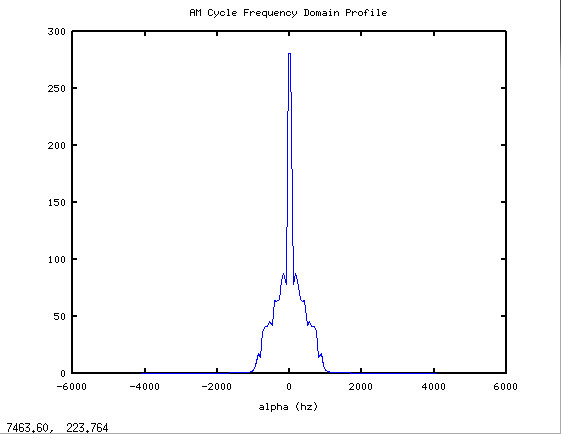
\includegraphics[width=\linewidth]{../img/Report_AM_Ia_Ideal.png}
  \caption{ }
\end{subfigure}
\begin{subfigure}{.49\textwidth}
  \centering
  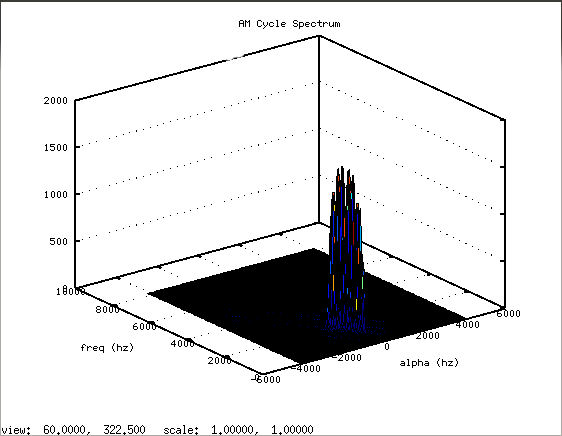
\includegraphics[width=\linewidth]{../img/Report_AM_Sxa_Ideal.png}
  \caption{ }
\end{subfigure}
\caption{Ideal Frequency Domain Profile (a) and Cycle Spectral Correlation (b)
for Amplitude Modulation}
\label{fig:IdealAMCyclo}
\end{figure}

\begin{figure}
\centering
\begin{subfigure}{.49\textwidth}
\centering
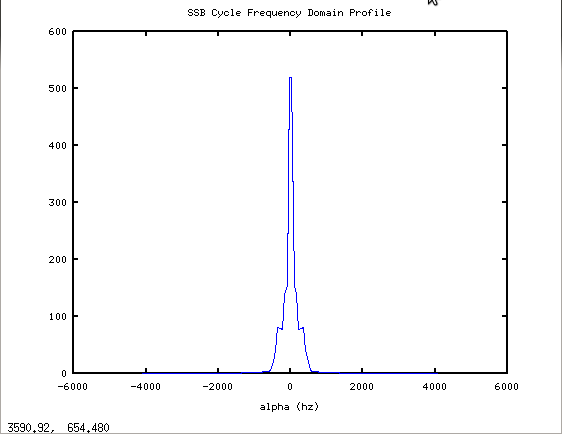
\includegraphics[width=\linewidth]{../img/Report_SSB_Ia_Ideal.png}
  \caption{ }
\end{subfigure}
\begin{subfigure}{.49\textwidth}
  \centering
  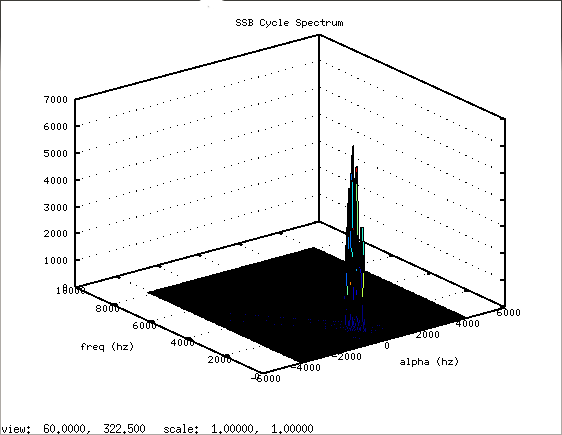
\includegraphics[width=\linewidth]{../img/Report_SSB_Sxa_Ideal.png}
  \caption{ }
\end{subfigure}
\caption{Ideal Frequency Domain Profile (a) and Cycle Spectral Correlation (b)
for Single Side Band Modulation}
\label{fig:IdealSSBCyclo}
\end{figure}

\begin{figure}
\centering
\begin{subfigure}{.49\textwidth}
\centering
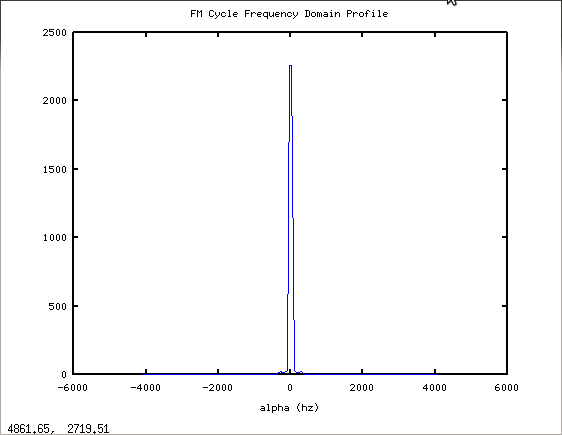
\includegraphics[width=\linewidth]{../img/Report_FM_Ia_Ideal.png}
  \caption{ }
\end{subfigure}
\begin{subfigure}{.49\textwidth}
  \centering
  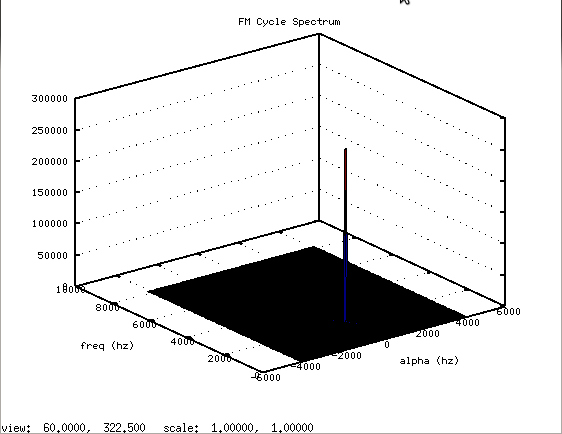
\includegraphics[width=\linewidth]{../img/Report_FM_Sxa_Ideal.png}
  \caption{ }
\end{subfigure}
\caption{Ideal Frequency Domain Profile (a) and Cycle Spectral Correlation (b)
for Frequency Modulation}
\label{fig:IdealFMCyclo}
\end{figure}

\begin{figure}
\centering
\begin{subfigure}{.49\textwidth}
\centering
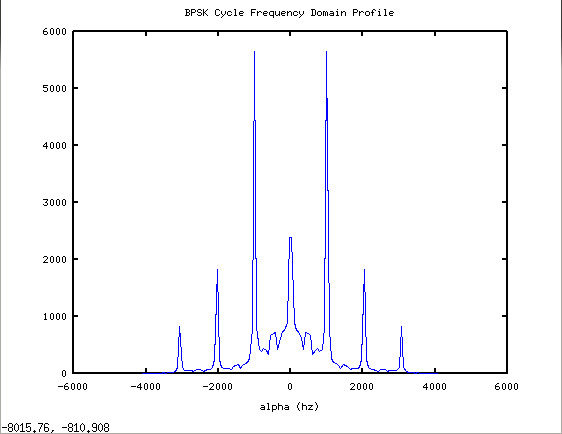
\includegraphics[width=\linewidth]{../img/Report_BPSK_Ia_Ideal.png}
  \caption{ }
\end{subfigure}
\begin{subfigure}{.49\textwidth}
  \centering
  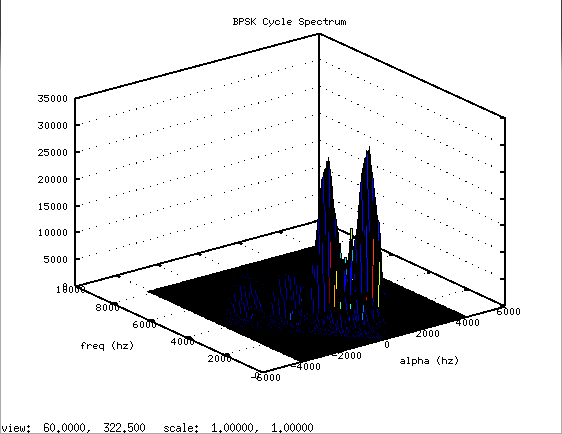
\includegraphics[width=\linewidth]{../img/Report_BPSK_Sxa_Ideal.png}
  \caption{ }
\end{subfigure}
\caption{Ideal Frequency Domain Profile (a) and Cycle Spectral Correlation (b)
for Binary Phase Shift Keying Modulation}
\label{fig:IdealBPSKCyclo}
\end{figure}


\begin{figure}
\centering
\begin{subfigure}{.49\textwidth}
\centering
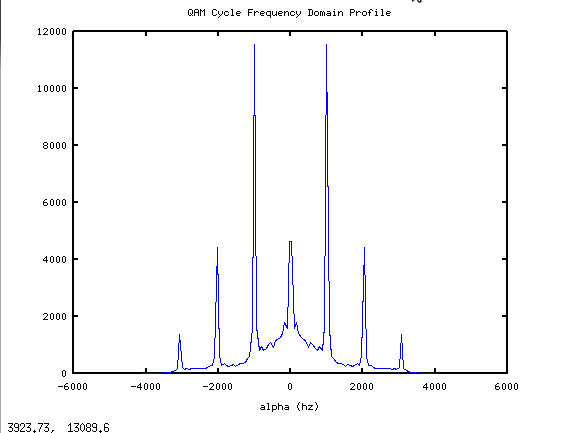
\includegraphics[width=\linewidth]{../img/Report_QAM_Ia_Ideal.png}
  \caption{ }
\end{subfigure}
\begin{subfigure}{.49\textwidth}
  \centering
  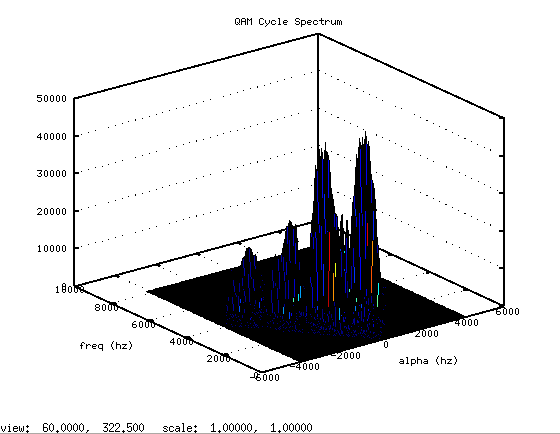
\includegraphics[width=\linewidth]{../img/Report_QAM_Sxa_Ideal.png}
  \caption{ }
\end{subfigure}
\caption{Ideal Frequency Domain Profile (a) and Cycle Spectral Correlation (b)
for Quadrature Amplitude Modulation}
\label{fig:IdealQAMCyclo}
\end{figure}

\begin{figure}
\centering
\begin{subfigure}{.49\textwidth}
\centering
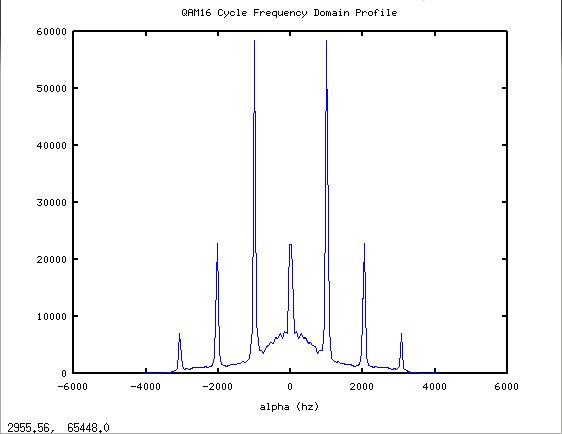
\includegraphics[width=\linewidth]{../img/Report_QAM16_Ia_Ideal.png}
  \caption{ }
\end{subfigure}
\begin{subfigure}{.49\textwidth}
  \centering
  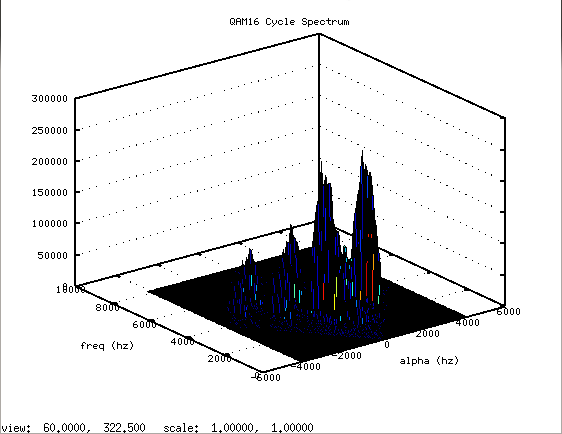
\includegraphics[width=\linewidth]{../img/Report_QAM16_Sxa_Ideal.png}
  \caption{ }
\end{subfigure}
\caption{Ideal Frequency Domain Profile (a) and Cycle Spectral Correlation (b)
for 16-Quadrature Amplitude Modulation}
\label{fig:IdealQAM16Cyclo}
\end{figure}

\begin{figure}
\centering
\begin{subfigure}{.49\textwidth}
\centering
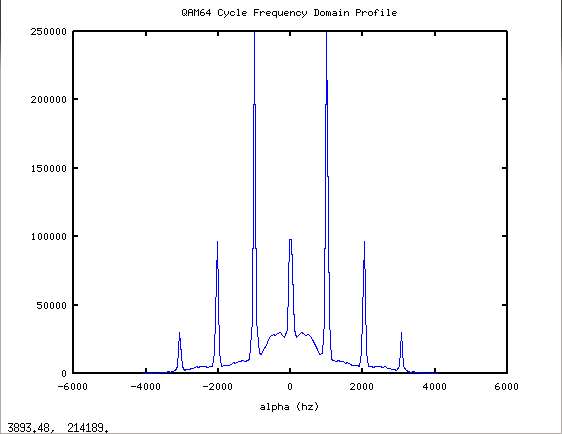
\includegraphics[width=\linewidth]{../img/Report_QAM64_Ia_Ideal.png}
  \caption{ }
\end{subfigure}
\begin{subfigure}{.49\textwidth}
  \centering
  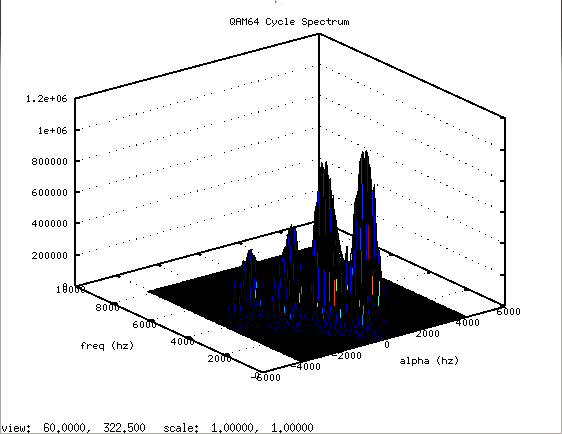
\includegraphics[width=\linewidth]{../img/Report_QAM64_Sxa_Ideal.png}
  \caption{ }
\end{subfigure}
\caption{Ideal Frequency Domain Profile (a) and Cycle Spectral Correlation (b)
for 64-Quadrature Amplitude Modulation}
\label{fig:IdealQAM64Cyclo}
\end{figure}


\begin{table}
\caption{Frequency Domain Profile Results}
\centering
\begin{tabular}{ l | c | c | c | c | c | c } \hline
SNR   &	 -3 &	 0 &	 3 &	 5 &	 10 &	 15\\ \hline \hline 
AM    &	 100 &	 100 &	 100 &	 100 &	 100 &	 100 \\ \hline 
 SSB   &	 0 &	 0 &	 0 &	 0 &	 0 &	 100 \\ \hline 
FM    &	 0 &	 0 &	 0 &	 0 &	 100 &	 100 \\ \hline 
BPSK  &	 0 &	 0 &	 0 &	 0 &	 2 &	 100 \\ \hline 
QAM   &	 3 &	 23 &	 44 &	 76 &	 100 &	 100 \\ \hline 
QAM16 &	 100 &	 100 &	 100 &	 100 &	 100 &	 100 \\ \hline 
QAM64 &	 0 &	 0 &	 0 &	 2 &	 99 &	 100 \\ \hline 
\end{tabular}
\label{tab:CycloHits}
\end{table}

\begin{table}
\caption{Frequency Domain Profile Results, False Positives}
\centering
\begin{tabular}{ l | c | c | c | c | c | c } \hline
SNR   &	 -3 &	 0 &	 3 &	 5 &	 10 &	 15\\ \hline \hline 
AM &	 28.6 &	 28.6 &	 28.6 &	 28.6 &	 14.3 &	 0.0 \\ \hline 
 SSB &	 0.0 &	 0.0 &	 0.0 &	 0.0 &	 0.0 &	 0.0 \\ \hline 
FM &	 0.0 &	 0.0 &	 0.0 &	 0.0 &	 0.0 &	 0.0  \\ \hline 
BPSK &	 0.0 &	 0.0 &	 0.0 &	 0.0 &	 0.0 &	 0.0 \\ \hline 
QAM &	 0.3 &	 0.0 &	 0.0 &	 0.1 &	 0.1 &	 0.0 \\ \hline 
QAM16 &	 42.1 &	 39.6 &	 36.6 &	 31.6 &	 14.0 &	 0.0 \\ \hline 
QAM64 &	 0.0 &	 0.0 &	 0.0 &	 0.0 &	 0.0 &	 0.0 \\ \hline
\end{tabular}
\label{tab:CycloFalsePos}
\end{table}
